\documentclass[10pt, a4paper]{amsart}
% \documentclass[10pt,showpacs,preprintnumbers,footinbib,amsmath,amssymb,aps,prl,twocolumn,groupedaddress,superscriptaddress,showkeys]{revtex4-1}
\usepackage[]{graphicx}
\usepackage[]{hyperref}
\usepackage[]{physics}
\usepackage[]{listings}
\usepackage[T1]{fontenc}
\usepackage{color}
\usepackage[ruled,vlined]{algorithm2e}

\usepackage{amsmath, amsfonts, amssymb}
\usepackage{listings}
\usepackage[]{subcaption}

\newcommand{\erfc}{\text{erfc}}

% Definition of code and how the code should look.
\usepackage{xcolor}
\definecolor{codegreen}{rgb}{0,0.6,0}
\definecolor{codegray}{rgb}{0.5,0.5,0.5}
\definecolor{codepurple}{rgb}{0.58,0,0.82}
\definecolor{backcolour}{rgb}{0.95,0.95,0.92}
\definecolor{mygreen}{rgb}{0,0.6,0}
\definecolor{mymauve}{rgb}{0.58,0,0.82}


\lstdefinestyle{python3}{
    backgroundcolor=\color{backcolour},
    commentstyle=\color{codegreen},
    keywordstyle=\color{magenta},
    numberstyle=\tiny\color{codegray},
    stringstyle=\color{codepurple},
    basicstyle=\ttfamily\footnotesize,
    breakatwhitespace=false,
    breaklines=true,
    captionpos=b,
    keepspaces=true,
    numbers=left,
    numbersep=5pt,
    showspaces=false,
    showstringspaces=false,
    showtabs=false,
    tabsize=2
}
% End def.



\lstset{ %
  backgroundcolor=\color{white},   % choose the background color; you must add \usepackage{color} or \usepackage{xcolor}
  basicstyle=\footnotesize,        % the size of the fonts that are used for the code
  breakatwhitespace=false,         % sets if automatic breaks should only happen at whitespace
  breaklines=true,                 % sets automatic line breaking
  captionpos=b,                    % sets the caption-position to bottom
  commentstyle=\color{mygreen},    % comment style
  deletekeywords={...},            % if you want to delete keywords from the given language
  escapeinside={\%*}{*)},          % if you want to add LaTeX within your code
  extendedchars=true,              % lets you use non-ASCII characters; for 8-bits encodings only, does not work with UTF-8
  frame=single,	                   % adds a frame around the code
  keepspaces=true,                 % keeps spaces in text, useful for keeping indentation of code (possibly needs columns=flexible)
  keywordstyle=\color{blue},       % keyword style
  language=python,                    % the language of the code
  style = python3,
  otherkeywords={*,...},           % if you want to add more keywords to the set
  rulecolor=\color{black},         % if not set, the frame-color may be changed on line-breaks within not-black text (e.g. comments (green here))
  showspaces=false,                % show spaces everywhere adding particular underscores; it overrides 'showstringspaces'
  showstringspaces=false,          % underline spaces within strings only
  showtabs=false,                  % show tabs within strings adding particular underscores
  stepnumber=2,                    % the step between two line-numbers. If it's 1, each line will be numbered
  stringstyle=\color{mymauve},     % string literal style
  tabsize=2,	                     % sets default tabsize to 2 spaces
}

\title[Problem set 3]{Problem set 3: Dissusion and Advection\\
\normalsize{Due: 3 Nov. 2020} \\
  \hrulefill\small{GEO2300: Fysiske prosesser i geofag }\hrulefill}

\author[Sundberg]{Sigurd Sandvoll Sundberg}
\date{\today}

\begin{document}
\maketitle

\section{Problem 1: Burgers Equation}
\subsection{a)}
An analytical solution to Burgers equation can look as follows 
\begin{equation}
	h = \frac{a}{2} - \frac{a}{2}\tanh(a\left(\frac{x-0.5at}{4\nu_t}\right))
\end{equation}

The following Python implementation using classes enables ut to call the calculate the analytical solution 
\lstinputlisting[firstline=16,lastline=26]{../code/1a.py}
\begin{figure}
	\centering
	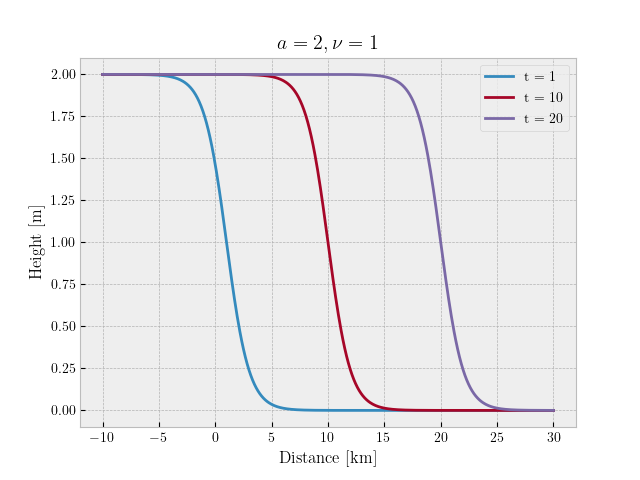
\includegraphics[width=0.9\textwidth]{../code/1a1.png}
	\caption{text}
	\label{key1}
\end{figure}
\begin{figure}
	\centering
	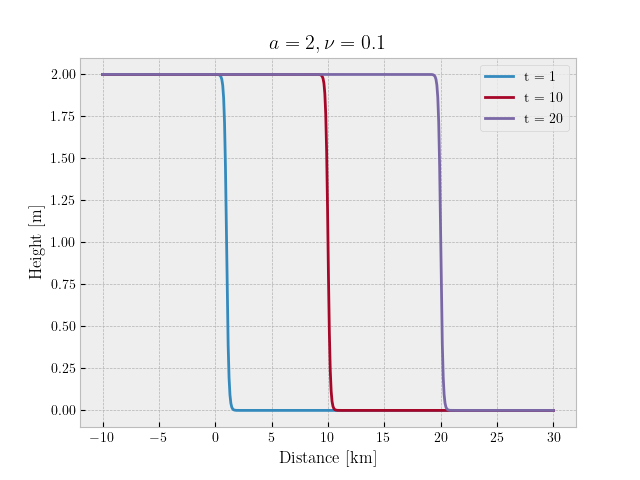
\includegraphics[width=0.9\textwidth]{../code/1a2.png}
	\caption{text}
	\label{key2}
\end{figure}
We can see from figure \ref{key1} and figure \ref{key2} that we are different wave behavior when we change the viscosity. For $\nu = 1$ we have waves which can be classified as smooth. 
Looking at the wave with $\nu = 0.1$, we see a steeper edge, almost right angled like. This would then resemble more of a wall rolling down the fjord, and less that of a wave. We can also see that the velocity of the two waves are roughly the same, with the middle of the wave being at the same point for both waves. 

On this note, we can also see that the bottom parts the wave in figure \ref{key1} is further ahead of the wave than the rest, making it "faster" than the wave in figure \ref{key2}. By this its meant that the bottom of the wave will be hitting areas of the shore quicker than that of the much steeper wave. 

\begin{figure}
	\centering
	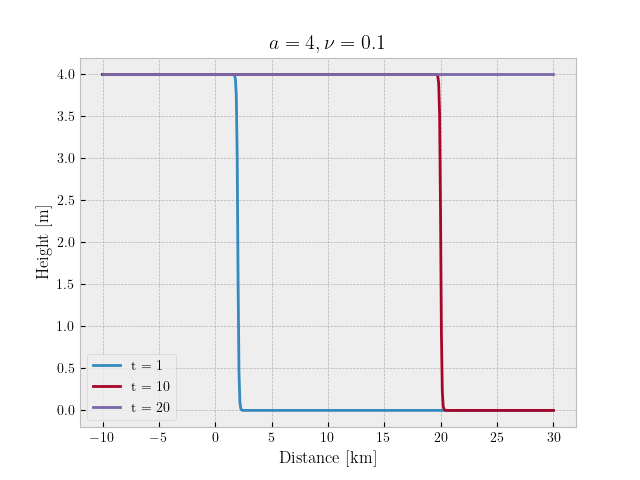
\includegraphics[width=0.9\textwidth]{../code/1a4.png}
	\caption{text}
	\label{key3}
\end{figure}
A wave with a large amplitude seen in figure \ref{key3}, have a higher velocity down the fjord. This can be seen as for the last timestep, we are not able to spot the wave itself, only the top of the wave. Resulting in a shorter available period for which you are able to evacuate the coast. 

\subsection{b)}
Burgers equation it self goes as follows 
\begin{equation}
	\frac{\partial }{\partial t}h + h\frac{\partial}{\partial x}h = \nu_t \frac{\partial^2}{\partial x^2}h
\end{equation}

We will discretize this equation and write it in finite difference form then matrix form using FTCS scheme. We then have the following equation 
\begin{equation}
	\frac{h_i^{n+1}- h_i^n}{dt} + h_j^n\frac{h_{j+1}^n-h_{j-1}^n}{2dx} = \nu_t\frac{h^n_{j+1} + h^n_{j-1} - 2h_j^n}{dx^2}
\end{equation}
However calculating the term $h\frac{\partial}{\partial x}h$, the advection terms is difficult and slow. We can however approximate this by using $E = h^2/2$, using the midpoint method. This gives us a new equation on the form 
\begin{equation}
		\frac{h_j^{n+1}- h_j^n}{dt} +\frac{E_{j+1}^n-E_{j-1}^n}{2dx} = \nu_t\frac{h^n_{j+1} + h^n_{j-1} - 2h_j^n}{dx^2}
\end{equation}

Re arranging this equation we have 
\begin{equation}
	h_i^{n+1} = sh_{j+1}^n + (1-2s)h_j^n + sh_{j-1}^n + c(E_{j-1}^n - E_{j+1}^n)
\end{equation}
with $s = (dt\nu_t)/(dx^2)$ and $c = dt/(2dx)$.
Our boundary conditions are given by $h(x=-10,t) = 2$ and $h(x=30, t) = 0$. Expanding our finite difference scheme for 5 grids points we have 
\begin{align}
	h_0 &= sh_1 + (1-2s)h_0 + sh_{-1} + cE_{-1} - cE_1\\
	&= sh_1 + (1-2s)h_0 + 2s + 2c - cE_1\\
	h_1 &= sh_2 + (1-2s)h_1 + sh_0 + cE_2 - cE_0\\
	h_2 &= sh_3 + (1-2s)h_2 + sh_1 + cE_3 - cE_1\\
	h_3 &= sh_4 + (1-2s)h_3 + sh_2 + cE_4 - cE_2\\
	h_4 &= sh_5 + (1-2s)h_4 + sh_3 + cE_5 - cE_3\\
	&= (1-2s)h_4 + sh_3 - cE_3
\end{align}
This makes us able to create the two following matrices
\begin{equation}
	A = 
	\begin{bmatrix}
		0 & -c & 0 & 0 & 0\\
		c & 0 & -c & 0 & 0\\
		0 & c & 0 & -c & 0\\
		0 & 0 & c & 0 & -c\\
		0 & 0 & 0 & c & 0 
	\end{bmatrix}
\quad 
B = 
\begin{bmatrix}
	1-2s & s & 0 & 0 & 0\\
	s & 1-2s & s & 0 & 0\\
	0 & s & 1-2s & s & 0\\
	0 & 0 & s & 1-2s & s\\
	0 & 0 & 0 & s & 1-2s
\end{bmatrix}
\end{equation}

Our matrix vector system then looks as follows 
\begin{equation}
	\vec{h} = \mathbf{A}\vec{E} + \mathbf{B}\vec{h} + \vec{b}
\end{equation}
where $\vec{b}$ is given by the boundary conditions. This is given by an zero vector of length n, with element $u_0 = 2s+2c$.

\subsection{c)}
The following Python implementation using Classes implements the FTCS scheme and a solver for Burgers equation.
\lstinputlisting[firstline=38, lastline=102]{../code/1b.py}
Implemented in the code is overflow handling for dealing potential overflows in $\vec{E}$, where they are the most prone as this is defined as the square of $\vec{h}$

\subsection{d)}
We will use the analytical solution at $h(x,t=1)$ as the initial condition. 
\begin{figure}
	\centering
	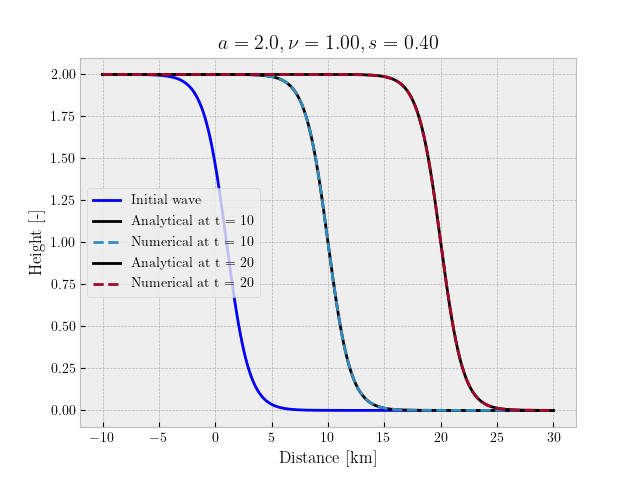
\includegraphics[width=0.9\textwidth]{../code/fig1.png}
	\caption{text}
	\label{key4}
\end{figure}
\begin{figure}
	\centering
	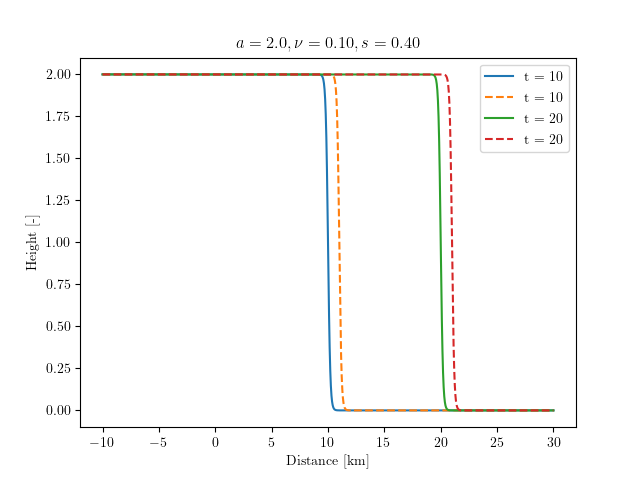
\includegraphics[width=0.9\textwidth]{../code/fig2.png}
	\caption{text}
	\label{key5}
\end{figure}
\begin{figure}
	\centering
	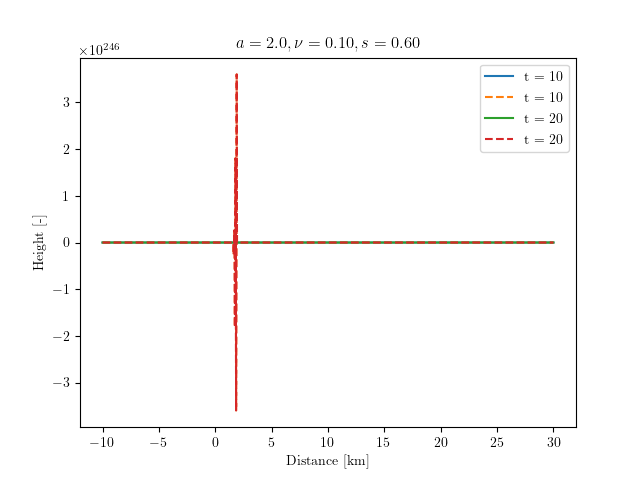
\includegraphics[width=0.9\textwidth]{../code/fig3.png}
	\caption{text}
	\label{key6}
\end{figure}

We see from both figure \ref{key4} and figure \ref{key5} that the numerical solution are on top of the analytical solutions, with no visible differences. Thus we can conclude that for our set of times for matrices of size $n = 750$ and $n=1500$, for $\nu = 1$ and $\nu=0.1$, respectively. 

Looking at figure \ref{key6} we see that we have no recognizable behavior as we encountered an overflow whilst calculating $\vec{E}$. This is expected as we have chosen $s = 0.6$, which is greater than the $s < 0.5$ which is required by the FTCS scheme for it to be stable. 
\section{Problem 2: Chaos}
\subsection{a)}
Given the following equation 
\begin{equation}
	\frac{d}{dt}u + ru^2 = ru - u.
\end{equation}

The map to this equation using $dt = 1$ looks as follows
\begin{equation}
u^{n+1} = ru(1-u)
\end{equation}

\subsection{b)}
The steady state value(s) for this map, as a function of r can be found by setting $du/dt =0$. which gives us $-ru^2 + ru - u= 0$. Solving this using the quadratic formula we end up with the following expression
\begin{equation}
u = \frac{(r-1)\pm (r-1)}{2r}
\end{equation}
which gives two solutions. 
\begin{equation}
	u = \left\lbrace\begin{split}
			&0,\\
			&1-1/r 
	\end{split} \right.
\end{equation}
\subsection{c)}
The following Python program using Classes implements all aspects of the chaos modeling we are doing. 
\lstinputlisting[firstline=18,lastline=102]{../code/2a.py}
This also has inbuilt error handling for dealing with overflows. 

\subsection{d)}
Firstly we are interested in when the system is at a steady state. A steady state is defined as $u^n = ru^n(1-u^n)$, equivalent to $du/dt = 0$. This follows a similar pattern as Markov Chains, as once we reach a steady state, we are not leaving the steady state, the system stay in the steady state. 

Trying to solve this problem has been annoying as there are no visible oscillation until you reach $r < 3$, however at zoom levels of around $10^{-20}$, there are visible oscillations prior to that, of amplitude equal to machine zero. 

Last solution that actually converges to a root is for r = 1. Seen in figure \ref{fig:1}
\begin{figure}
	\centering
	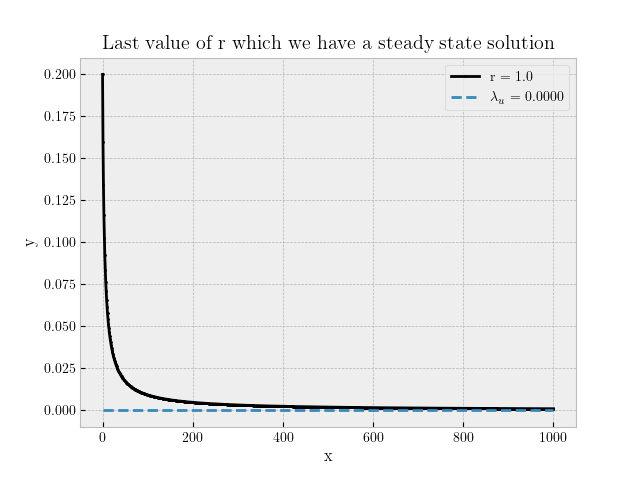
\includegraphics[width=0.9\textwidth]{../code/d.png}

	\caption{Last convergance to a root.}
		\label{fig:1}
\end{figure}
I assume that is what is asked for in this problem. However as stated, no visible oscillations where actually found until $r\geq3$.
Zero is the root in all cases. The range can be written either as $r\in[0,1)$ or $r\in[0,3)$. 
\subsection{e)}
Same follows for this, if we assume that we have oscillations that are invisible to the naked eye, unless heavily zoomed, the range is $r\in[1,3.5)$ or if we only care about  visible oscillations we have $r\in[3,3.5)$. 
\begin{figure}
	\centering
	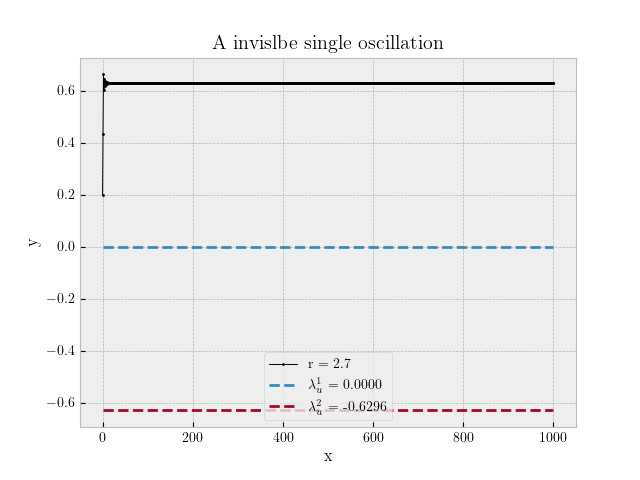
\includegraphics[width=0.9\textwidth]{../code/e1.png}

	\caption{Invisible single oscillation.}
		\label{fig:2}
\end{figure}
\begin{figure}
	\centering
	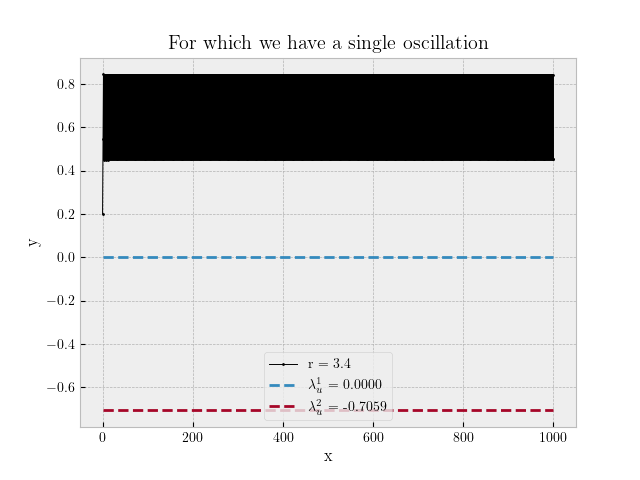
\includegraphics[width=0.9\textwidth]{../code/e2.png}

	\caption{Naked eye visible single oscillations.}
		\label{fig:3}
\end{figure}

Both figure \ref{fig:2} and figure \ref{fig:3} have single oscillations in them, however in figure \ref{fig:2} it is so small, that it is just above machine zero. 

\subsection{f)}
For a double oscillation see figure \ref{fig:4}.
\begin{figure}
	\centering
	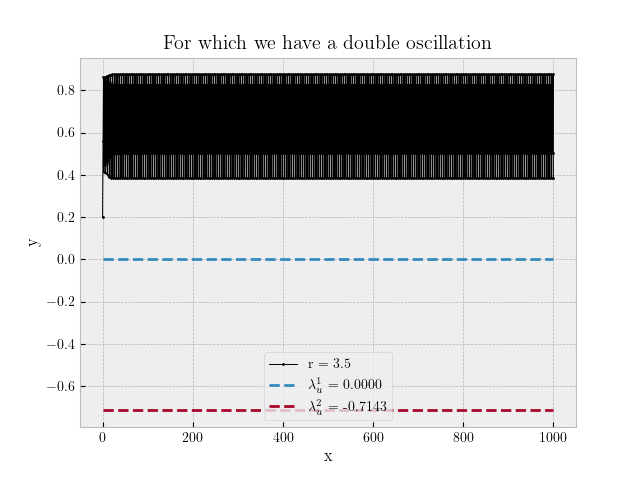
\includegraphics[width=0.9\textwidth]{../code/f2.png}

	\caption{Naked eye visible double oscillations.}
		\label{fig:4}
\end{figure}

\subsection{g)}
The found range for which we have chaos is $r\in[3.6,4.1)$. The min and max values of u vary, but for $r = 4.0$, they are respectively, 0 and 1. A plot of the chaos is seen in figure \ref{fig:5}.
\begin{figure}
	\centering
	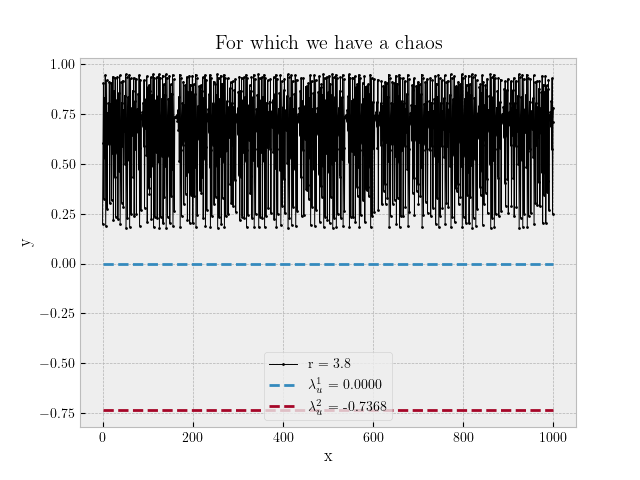
\includegraphics[width=0.9\textwidth]{../code/f.png}

	\caption{Chaos plot.}
		\label{fig:5}
\end{figure}

\subsection{h)}
For $r\in[4.1,\infty)$ we have an numerically unstable mapping.
An example is in figure \ref{fig:6}.
\begin{figure}
	\centering
	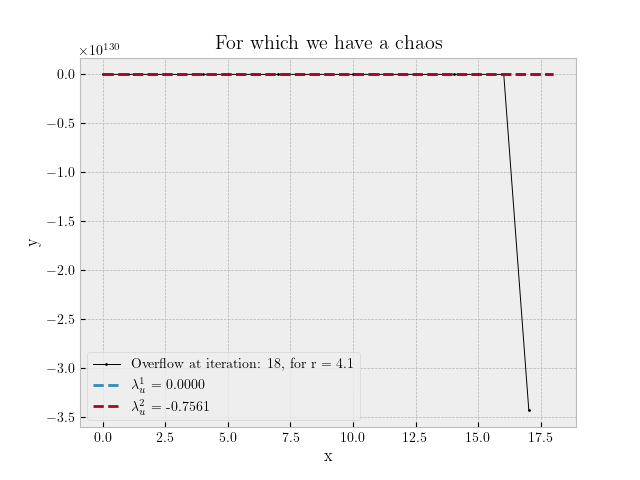
\includegraphics[width=0.9\textwidth]{../code/g.png}

	\caption{Numerically unstable.}
		\label{fig:6}
\end{figure}

\end{document}
